\chapter{Storia dei linguaggi di programmazione}

\section{Introduzione}

L'idea di "linguaggio di programmazione" emerge per far fare al compilatore determinati
compiti. Ogni computers, per quanto sofisticato comprende solo il concetto di bit, ma
per gli esseri umani è difficile esprimersi in quei termini. Per questo motivo si è
pensato di creare un linguaggio che fosse più vicino alla nostra comprensione. Con il
tempo si sono succedute molte idee e c'è stata una selezione naturale dei linguaggi. Alla fine
i linguaggi veramente importanti sono poco più di una decina.

\nt{Ai giorni nostri si da per scontata l'idea di linguaggio, ma neggli anni '40, Von Neumann
affermava di non vederne l'utilità.}

All'inizio si riteneva che nessuno avrebbe deciso di scrivere un programma in un linguaggio
perchè sarebbe stato troppo lento rispetto allo scrivere un programma in assembler, ma oggi 
quest'idea è superata per via dei sempre più efficienti compilatori.

Ripercorrendo la storia dei sistemi di calcolo si ha una prima idea con l'analytical
engine di Babbage, con Ada Lovelace che scrive il primo programma per questa macchina.
Successivamente con ENIAC si ha il primo computer elettronico (che poteva essere riconfigurato), ma il primo linguaggio
di programmazione è il Plankalkul di Konrad Zuse, che però non è mai stato implementato.
Nel Mark I Di Aiken le istruzioni erano codificate su nastro perforato. Tra il '43 e il '45
Goldstine e Von Neumann sviluppano il concetto di "flow chart" in cui si ha "=" interpretato come 
assegnamento.  Nel '48 il Manchester SSEM usa a 32 switch per stabilire il valore di un bit.
Nell’EDVAC, i bit che componevano il programma (scritto in
linguaggio macchina) e i dati, tutti rappresentati in binario, erano
inseriti uno a uno nelle Mercury Delay Lines. 

\dfn{Initial order}{Nel EDSAC nasce per la prima volta l'idea
"initial order": il codice di una determinata istruzione era associato a una lettera assegnata
in modo mnemonico (per esempio "S" significava subtract). Un istruzione macchina era costituita
da un tre caratteri di 5 bit ciascuno.}

\nt{Nell'initial order il programma era codificato su un nastro perforato. Era una sorta di
antenato del linguaggio assembler.}

\begin{figure}
    \centering
    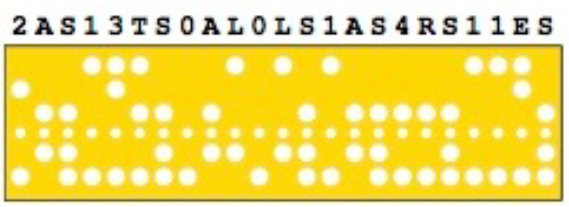
\includegraphics[scale = 0.3]{images/Initial order.png}
    \caption{Initial order}
    \label{fig:Initial order}
\end{figure}

\paragraph{In sostanza:}

\begin{itemize}
    \item Alla fine degli anni '40 c'erano poche decine di programmatori e meno di 20 computers;
    \item Non esistevano corsi/tutorial di programmazione;
    \item Erano stati scritti pochi programmi.
\end{itemize}

\dfn{Short code}{Lo short code viene implementato nel '49 da Maurice Wilkes. Si tratta di un linguaggio
che permette di scrivere programmi in modo più semplice. Veniva assegnato uno specifico numero a 6 bit
per indicare variabili e simboli di un'equazione. Si scrisse anche un programma per il calcolo delle
equazioni da calcolare (una sorta di primitivo interprete).
}

Tra il 1948 e il 1950 Haskell Curry sviluppa la programmazione strutturata.
Tuttavia Curry non considerava la fase di analisi sintattica

\section{Gli anni '50}

\dfn{For}{Il costrutto for viene introdotto nel '51 da Rutishaur.
La sua idea permetteva di generare codice rilocabile.}

Nel 1950 l'italiano Corrado Böhm concepisce un linguaggio di alto livello e un metodo di traduzione in 
linguaggio macchina. Nel suo lavoro:

\begin{itemize}
    \item Vengono introdotti "if then else" e "goto";
    \item Gli statement di assegnamento;
    \item Le subroutine;
    \item Un compilatore scritto nello stesso linguaggio dei programmi che deve tradurre.
\end{itemize}

Il compilatore di Böhm genera codice proporzionalmente al numero di passi da eseguire. Inoltre il linguaggio
di Böhm è universale (tuttavia è solo su carta).

\subsection{AUTOCODE}

\dfn{AUTOCODE}{
Il primo compilatore degno di questo nome viene svippato nel 1953 da Alick Glennie che noto che si poteva
usare lo stesso computer per tradurre un programma e far girare il programma sullo stesso computer. AUTOCODE
era complicato e il suo compilatore era composto da 750 istruzioni.}

AUTOCODE:

\begin{itemize}
    \item Rendeva più veloce e semplice la programmazione;
    \item Costituiva una perdita di efficienza del 10\% rispetto al linguaggio macchina.
\end{itemize}

Ma il lavoro di Glennie non ebbe il successo sperato poichè in quegli anni il focus non era tanto sullo scrivere un programma
ma sul fatto che i calcolatori si rompessero continuamente.

Negli anni '50 si sviluppa l'idea di pseudo-codice e si parlava di automatic coding invece che di compilatori.

\subsection{Gli anni dal '54 al '56}

In queglu anni si stava tenendo il SIMATIC (Symposium on the Mechanization of Thought Processes) in cui si discuteva
delle proprie scoperte.

\begin{itemize}
    \item Nel 1954 si sviluppa il primo assembler moderno, il SOAP;
    \item Tra il 1954 e il 1956 alla Boeing Airplane Company di Seattle
    viene sviluppato il sistema BACAIC, in cui espressioni algebriche
    vengono tradotte in subroutine di linguaggio macchina;
    \item Enton
    Elsworth lavora ad un sistema per la traduzione di equazioni
    algebriche in linguaggio macchina (dell’IBM 701), e chiama il suo
    sistema Kompiler;
    \item Viene messo a punto ADES, il primo linguaggio di programmazione imperativo;
    \item Nel 1956 , per IBM 650, viene sviluppato il compilatore IT.
\end{itemize}

\dfn{IT}{IT funzionava in due fasi:
\begin{enumerate}
    \item Veniva generato codice assembler intermedio;
    \item Da quel codice veniva generato codice macchina
\end{enumerate}
IT permetteva di scrivere in un linguaggio semplice con un'implementazione efficiente.}

\subsection{Il FORTRAN}

\dfn{FORTRAN}{Nel 1957 il FORTRAN fa la sua comparsa. All'inizio del 1954 John Backus,
Harlan Herrick e Irving Ziller iniziano a lavorare su un linguaggio di programmazione. 
In quegli anni i programmi venivano scritti o in assembler o in linguaggio macchina, per
cui non si pensava che il FORTRAN potesse avere successo.}

\paragraph{Specifiche:}

\begin{itemize}
    \item Sarebbe dovuto essere facile scrivere programmi in FORTRAN e sarebbe dovuto essere
    efficiente;
    \item Sarebbe dovuto essere facile da imparare;
    \item Non doveva essere svincolato dall'hardware (in quanto linguaggio di IBM).
\end{itemize}

Il manuale del FORTRAN aveva una grafica professionale, ma era pieno di errori e incompleto.
Tuttavia il FORTRAN influenzo la maggior parte dei linguaggi successivi e fino agli anni '70
fu utilizzato come standard per applicazioni scientifiche.

\subsection{LISP}

\dfn{LISP}{Nel 1958 fa il suo debutto il LISP. Fu il primo dei linguaggi funzionali. Nasce per la manipolazione
di espessioni simboliche con l'uso del concetto di "ricorsione". Inoltre il LISP usava sia liste che alberi.
Offriva un garbage collector e un sistema di tipi dinamico. Permetteva la meta-programmazione.}

\begin{itemize}
    \item Viene usata una notazione polacca (prefissa);
    \item Alcuni operatori potevano venire implementati direttamente in linguaggio macchina.
\end{itemize}

\nt{Alcune parti di LISP erano codificate in FORTRAN}

In LISP tutto veniva rappresentato da liste concatenate. La lista concatenata a destra è la rappresentazione interna
dei dati.

\subsection{COBOL}

\dfn{COBOL}{}